\begin{document}
%=================================================================
%                           Start Document
%=================================================================
\section{Implementation}
\lhead{Implementation} % section header
\setstretch{1.6}
\lhead{Implementation - Software Refactoring}
\subsection{Software Refactoring}
As mentioned introduction wise this project builds upon the work and code base originally developed for FES with the LegoPress \cite{olivier_legopress_2014} and further developed by a previous student. However the code quality was poor with thousands of lines of code and multiple functionalities all implemented in one file and one class. Therefore before continuing on with the project a proper refactoring of the code was necessary. The goal being to save time in the long run by creating modular, robust, readable code that could later be further built upon for use in clinical trials.

The software is written in C++ in QT.

\subsubsection{Documentation}

In order to understand the code it was decided that the first step would be to create documentation, specifically graphical representations of the interactions and hierarchy. To accomplish the code was documented and edited so that it would be compatible with doxygen. Doxygen is a documentation generation tool that automatically creates software documentation from annotated source code in HTML.

\begin{figure} [H]
    \centering
    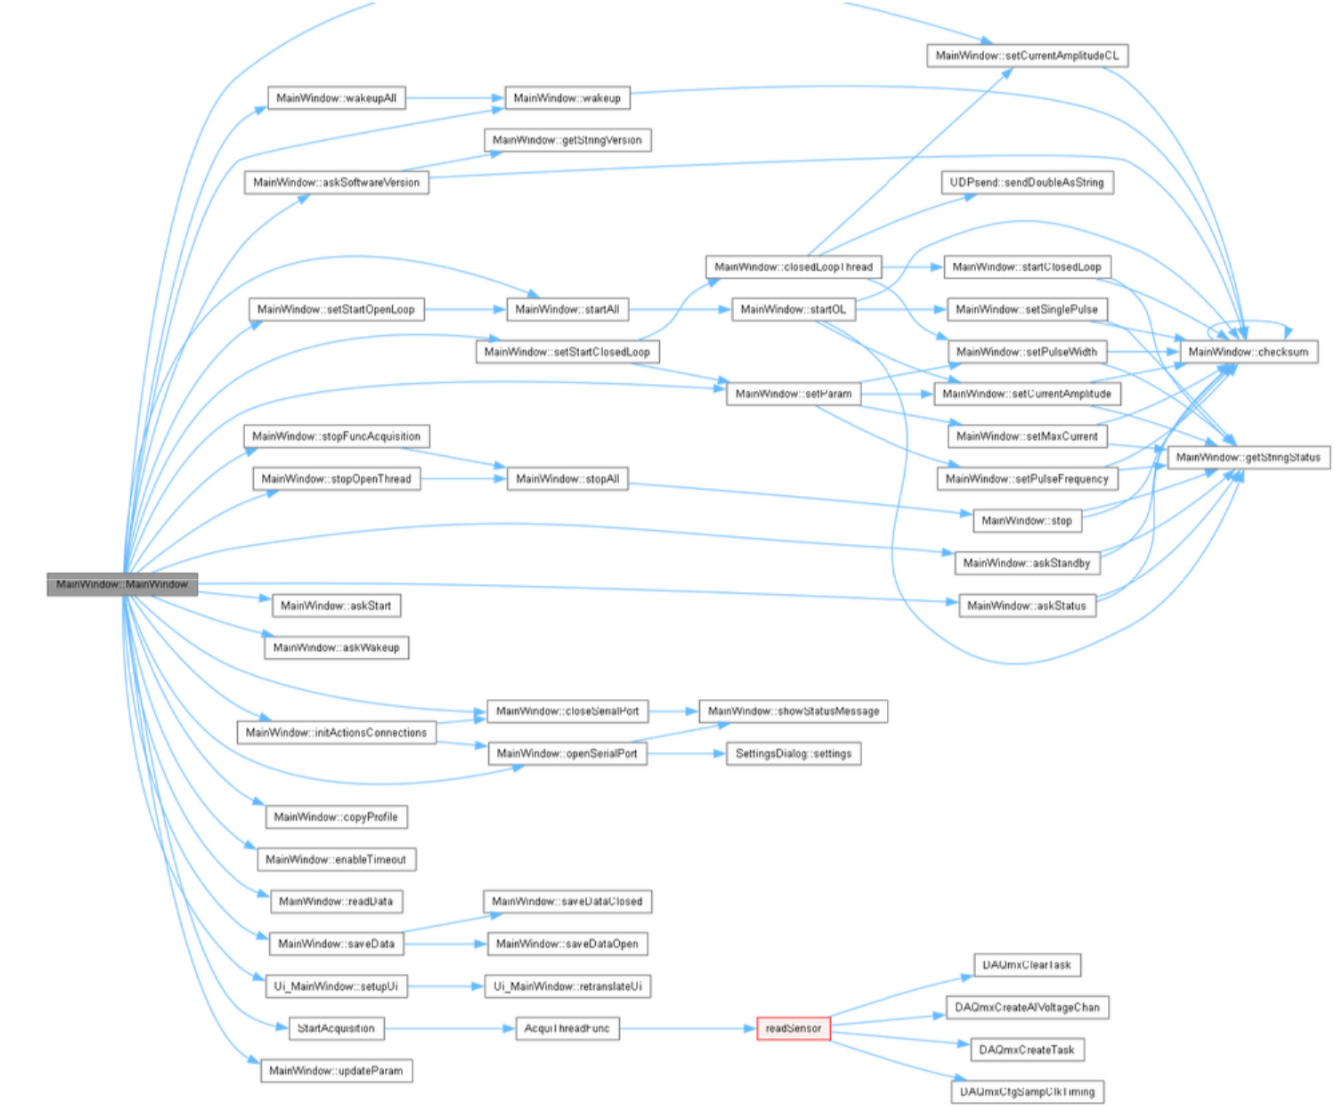
\includegraphics[width=0.9\linewidth]{images/oldDoxy.png}
    \caption{Original callgraph for mainwindow function before refactoring, generated by doxygen}
    \label{fig:oldDoxy}
\end{figure}

After the code had been documented and visualized in doxygen it became possible to see the call graphs and interactions such as in figure \ref{fig:oldDoxy}. This sped up the process of understanding the code thus laying important groundwork for the clearning and modularization step.

\subsubsection{Modularization}
In order to improve the code quality, a modularization and cleaning of the code base was necessary. The code was refactored and divided into classes based mainly on the code quality principles laid out in Code Complete by Steve McConnel \cite{steve_mcconnell_code_nodate}. This includes having clearly defined, minimal interfaces. This is accomplished by using the signal slot mechanism inbuilt into QT, which allows for communication between objects in an event-driven, decoupled manner. Another core concept is organizing modules hierarchically, where higher-level modules depend on lower-level modules but not the reverse. 

\begin{figure} [h]
    \centering
    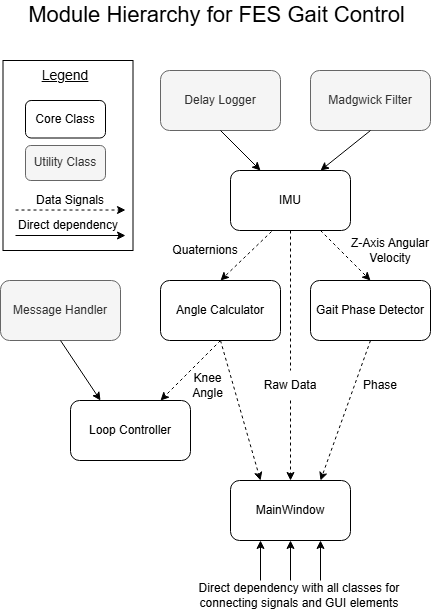
\includegraphics[width=0.6\linewidth]{images/gaitcontrol.png}
    \caption{Module hierarchy after refactoring}
    \label{fig:modulehier}
\end{figure}

A visualization of the hierarchy after refactoring can be seen in figure \ref{fig:modulehier} and description of each class are in table \ref{tab:class-overview}. Previously, all loop controller and IMU functionality and serial communication and bit handling was all done in the mainwindow class. There was also code only relevant for the legopress still in the mainwindow class. That code for the legopress was removed and the usable, existing code was moved to their appropriate classes which were the message handler, LoopController and MainWindow. All old IMU functionality was also removed since part of the project involved changing out the old wired IMUs with the new wireless IMUs developed in the lab. The final architecture has a high cohesion and low coupling resulting in readable, scalable, testable and reusable code.


\lhead{Implementation - Functional Electrical Stimulation Setup}
\subsection{Functional Electrical Stimulation Setup}

\subsubsection{Hardware}
The hardware used for the functional electrical stimulation was the StimWave developed at the REHassist lab. It consists of 10 channels where each channel is controlled via an RS-232 line in a master/slave manner. Each electrostimulation channel (slave) has its own adress and every command from the FES Gait Control software (master), is dedacted to only one channel. Meaning that each channel can be used in order to apply FES to a muscle. There is a protocol that describes what each 3 byte command encodes. Using this encoding the pulse frequency, pulse width and current amplitude may be adjusted. Along with other commands such as start, stop and status commands. 

\begin{figure} [h]
    \centering
    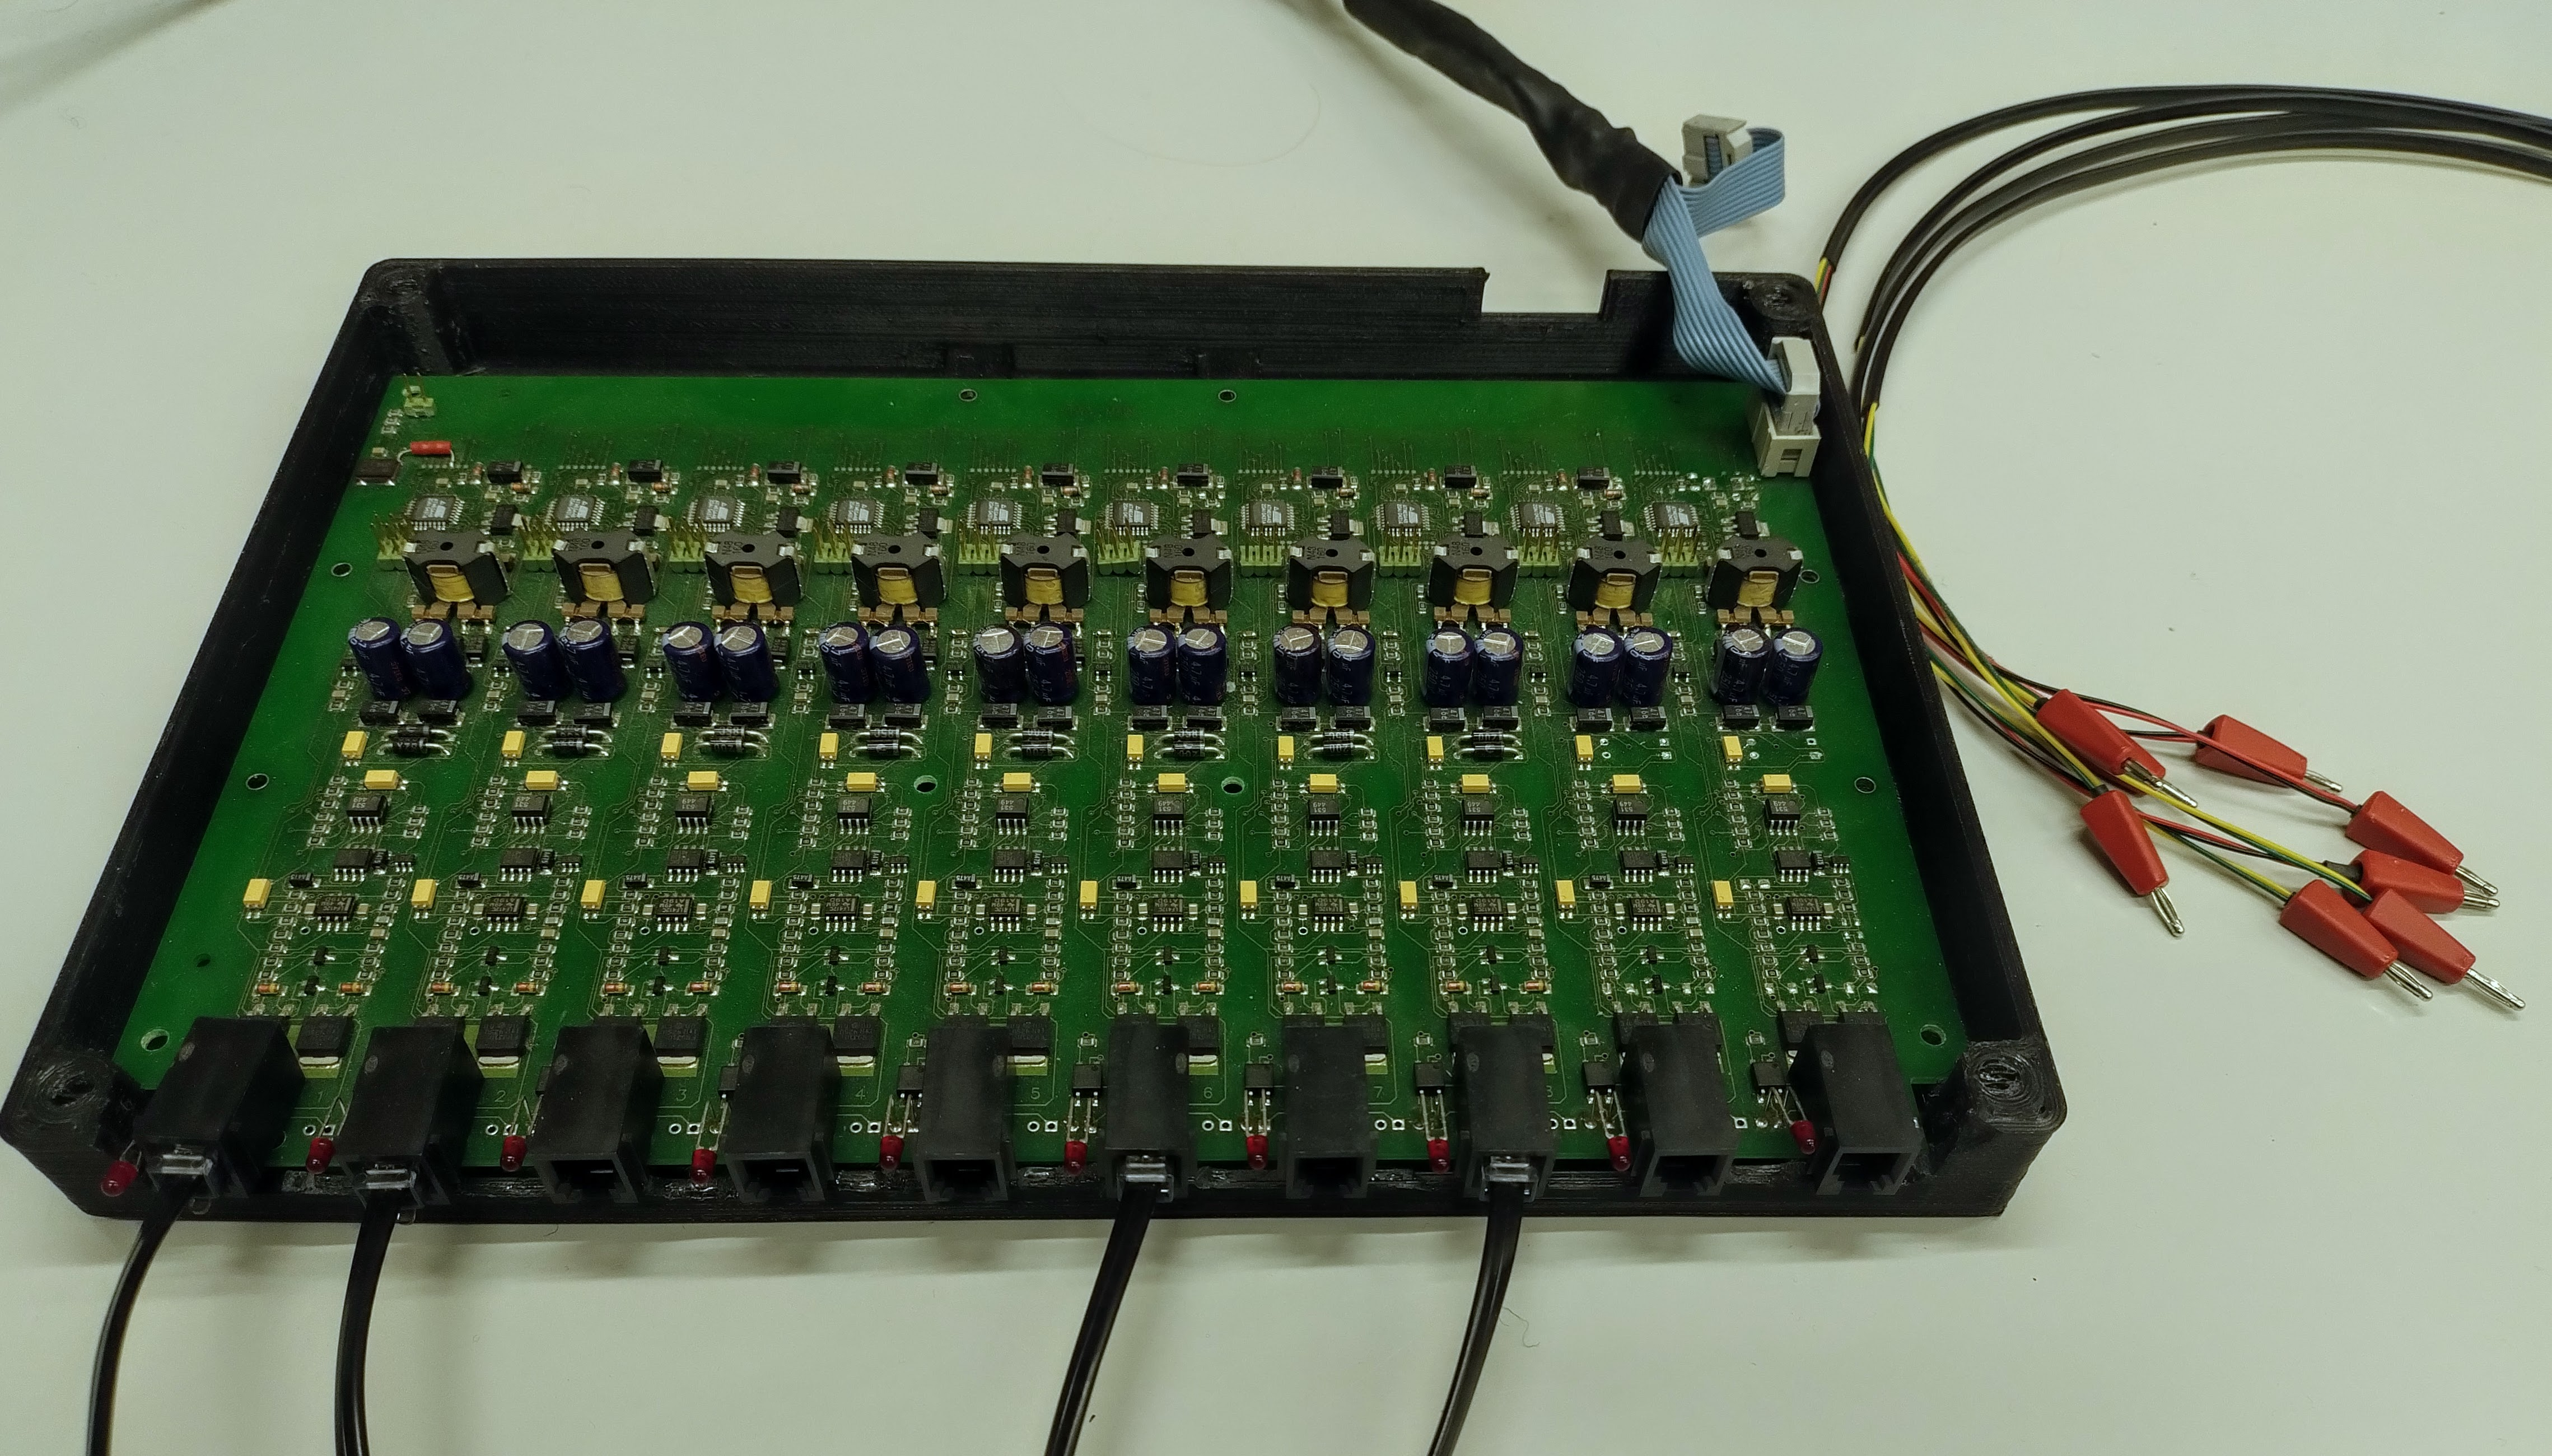
\includegraphics[width=0.8\linewidth]{images/stimwave.jpg}
    \caption{StimWave hardware used}
    \label{fig:stimwave}
\end{figure}

However the selection code for the pulse width and frequency had been changed since the implementation used in the original code base. The first step before using this hardware for FES was therefore to adjust the translation of pulsewidth and frequency to the correct 7 bit selection code thereby creating the correct 3 byte commands in the \texttt{MessageHandler} class. These changes were verified by using an oscilloscope before moving on to FES. 


\subsubsection{Stimulation waveform}
Stimulus waveforms are generally monophasic or biphasic. Monophasic waveforms consist of a single phase of electrical current delivered in one polarity, while Biphasic waveforms consist of a cathodic phase followed by an anodic phase. This mitigates the buildup of charge at the electrode-tissue interface by ensuring that the net charge delivered over time is zero, effectively reducing the risk of tissue damage as compared to monophasic waveforms \cite{peckham_functional_2005}. The biphasic rectangular stimulation is the most commonly used, as it offers the best force-amplitude ratio
\cite{lynch_functional_2008}. For these reasons the balanced biphasic rectangular waveform was chosen for the stimulation protocol.
 \begin{figure} [H]
     \centering
     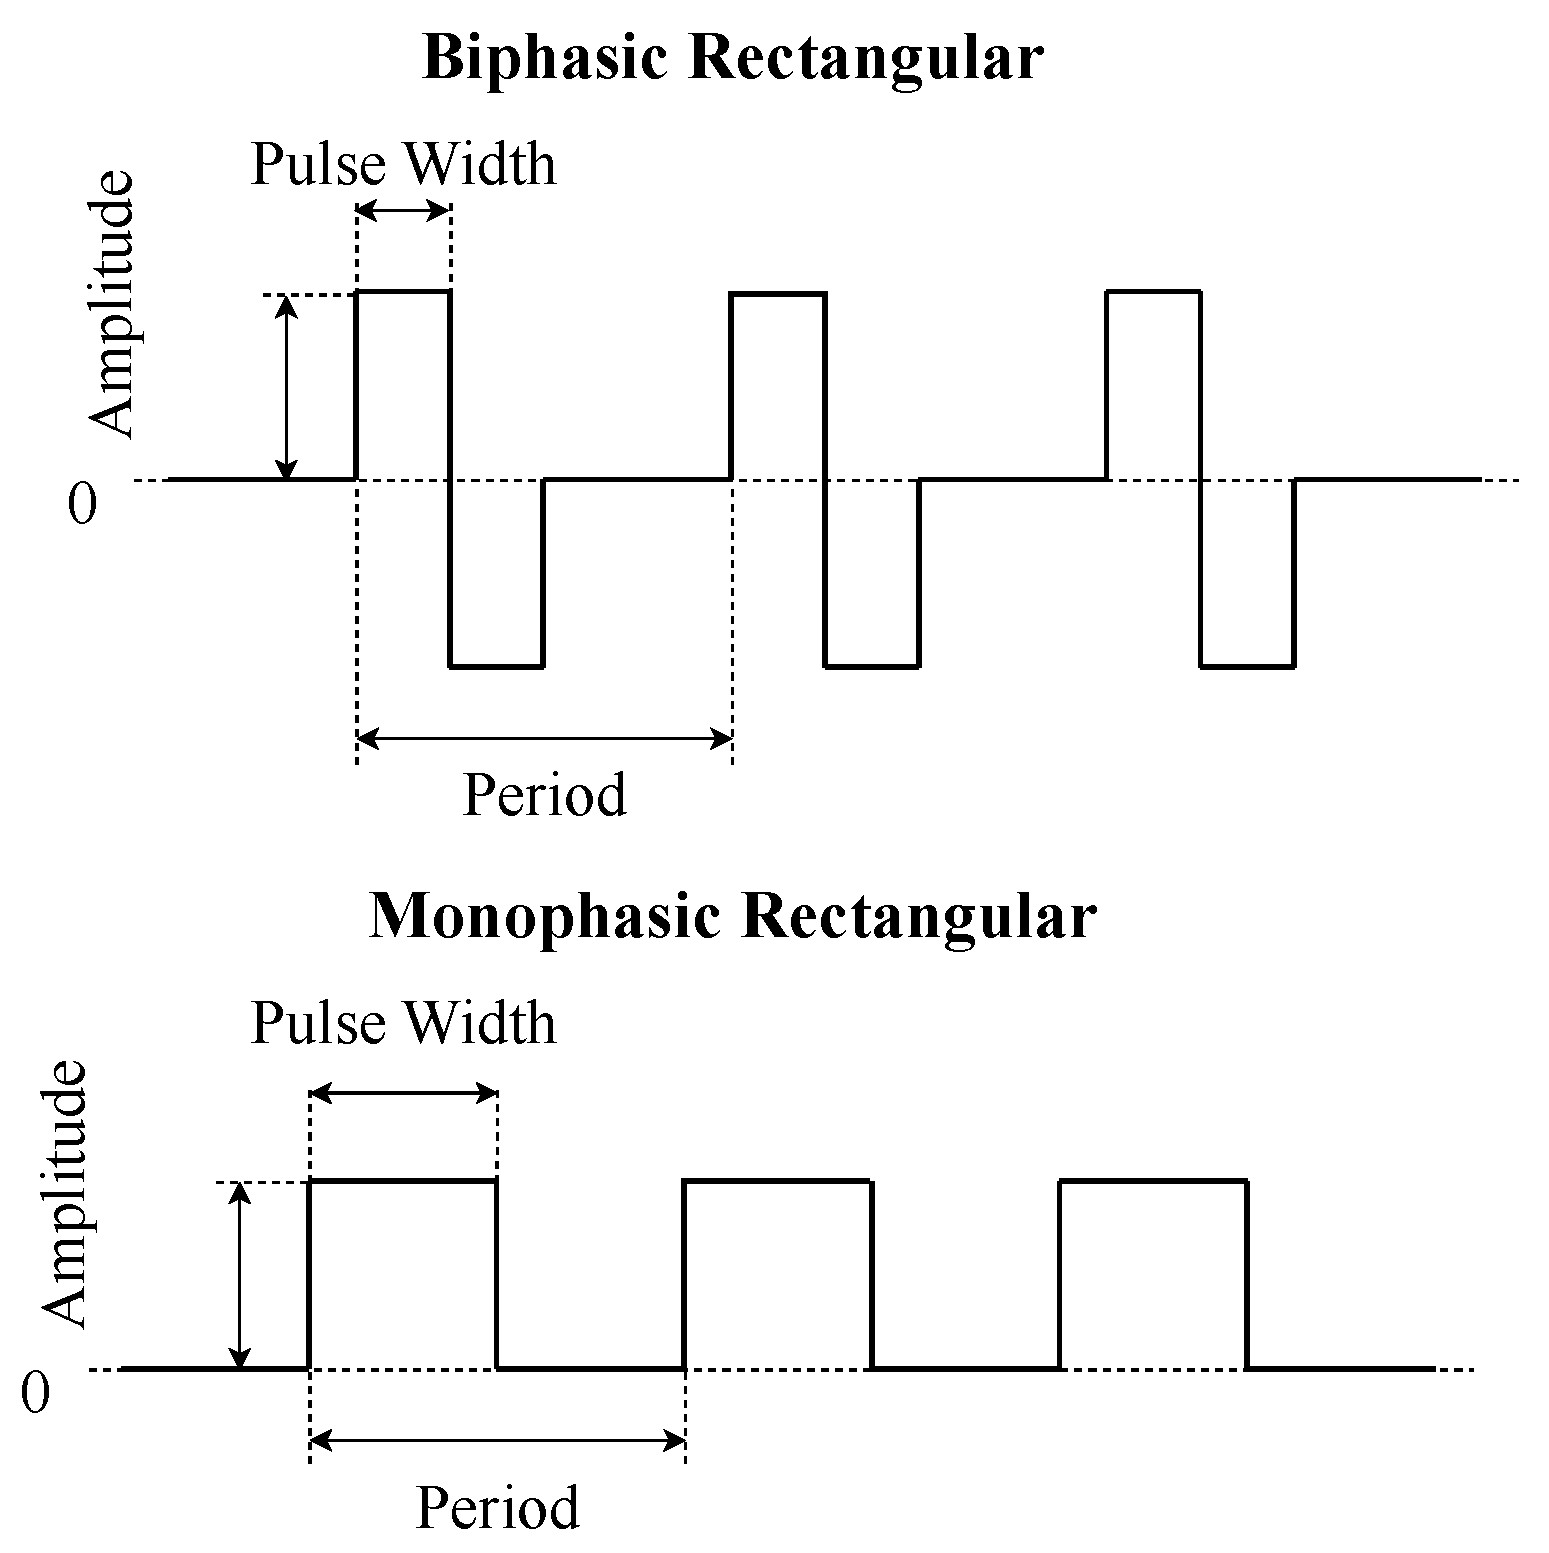
\includegraphics[width=0.6\linewidth]{images/twowaveform.jpg}
     \caption{Caption}
     \label{fig:enter-label}
 \end{figure}
 

\subsubsection{Stimulation frequency}
The stimulation frequency affects the strength of the contraction and its quality. A higher frequency will lead to the force produced by each subsequent pulse being added so that the mean force of the contraction is greater than that produced by a single twitch. Further increase in frequency results in sustained contraction which produces a smooth movement instead of individual twitches. The minimum frequency required to induce fairly consistent contraction is between 16 and 20 Hz \cite{marquez-chin_functional_2020}. A smoother contraction is also more comfortable for the patient. However one should not use a higher frequency than necessary since it has been observed that fatigue accumulated in a muscle is related to the number of pulses received \cite{bigland-ritchie_muscle_2000}. 

\begin{figure} [H]
    \centering
    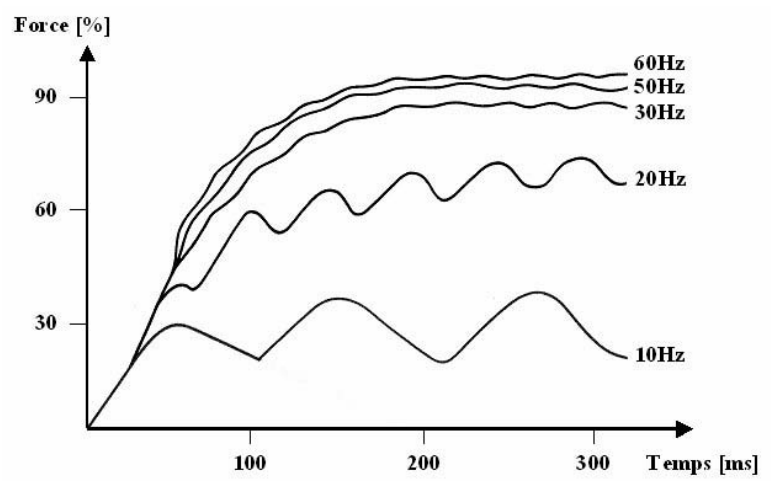
\includegraphics[width=0.7\linewidth]{images/stimfreq.png}
    \caption{Effect of stimulation frequency on force generation \cite{metrailler_systeme_2005}}
    \label{fig:stimfreq}
\end{figure}

When choosing the stimulation frequency the aim was therefore to choose the lowest frequency that still produced sustained contractions. In a clinical environment, the typical range of frequencies is around 20-50Hz, and during literature review it was observed that the majority of teams using FES on gait are using a stimulation frequency around 40Hz \cite{aout_effects_2023}. Therefore the same 40Hz stimulation frequency was chosen for this project.



\subsubsection{Stimulation intensity }
The stimulation intensity is determined by the pusle duration as well as the pulse amplitude. To vary the intesity one is therefore often kept constant while the other is tuned. 

 \todo{explain better why modulating w amplitude?} 
The pulse duration (pulse width) is the timespan of the stimulation pulse. Higher pulse widths result in more pronounced contraction and enable deeper tissue penetration of the stimulation . Most sudies attempting FES for gait employ pulse widths spanning from 200 to 400 \micro s. The majority keep the pulse duration fixed at 300 \micro s and only vary the amplitude in order to set the stimulation intensity.\cite{aout_effects_2023}

The amplitude of the stimulation determines which muscles are contracted and the strength of the contraction \cite{marquez-chin_functional_2020}. Larger amplitudes a larger proportion of the muscle fibers, including those located deeper. 

There are several clinically important values for the amplitude that can be identified. The first is the motor threshold, which is the minimum intensity  that results in a visible muscle contraction, even if it does not produce a movement \cite{marquez-chin_functional_2020}. The second is the Maximum tolerable intensity, which is the maximum amplitude that the person can sustain without pain. Finally there is the operational stimulation amplitude, which is the amplitude that produces the intended functional movement needed for the gait cycle. 

These thresholds are highly variable and dependent on both muscle and subject, therefore they are determined here experimentally by slowly ramping up the amplitude for one muscle at a time. Noting when a motor threshold is reached, when the maximum tolerable intensity is reached and based on these values and feedback from the patient a operational stimulation amplitude is set somewhere between the thresholds. This is expanded upon in the sections relating to the open loop and closed loop implementations.

\todo{picture of GUI}

\subsubsection{Electrode configuration}
There are two main configuration for electrical activation of neuromuscular tissue. There is bipolar stimulation in which each stimulation cite has an active electrode placed near the peripheral nerve and a reference electrode close by. The other configuration is monopolar where the return electrode is placed in a remote area near less excitable tissue \cite{peckham_functional_2005}. 
This approach reduces the number of leads and electrodes required, however for multichannel systems bipolar stimulation may allow greater selectivity of activation because each electrode par creates a more localized electric field \cite{grandjean_recruitment_1986}. For this reason and also since there were already cables compatible with this configuration available bipolar stimulation was chosen.
\begin{wrapfigure}{r}{0.3\textwidth} 
    \centering
    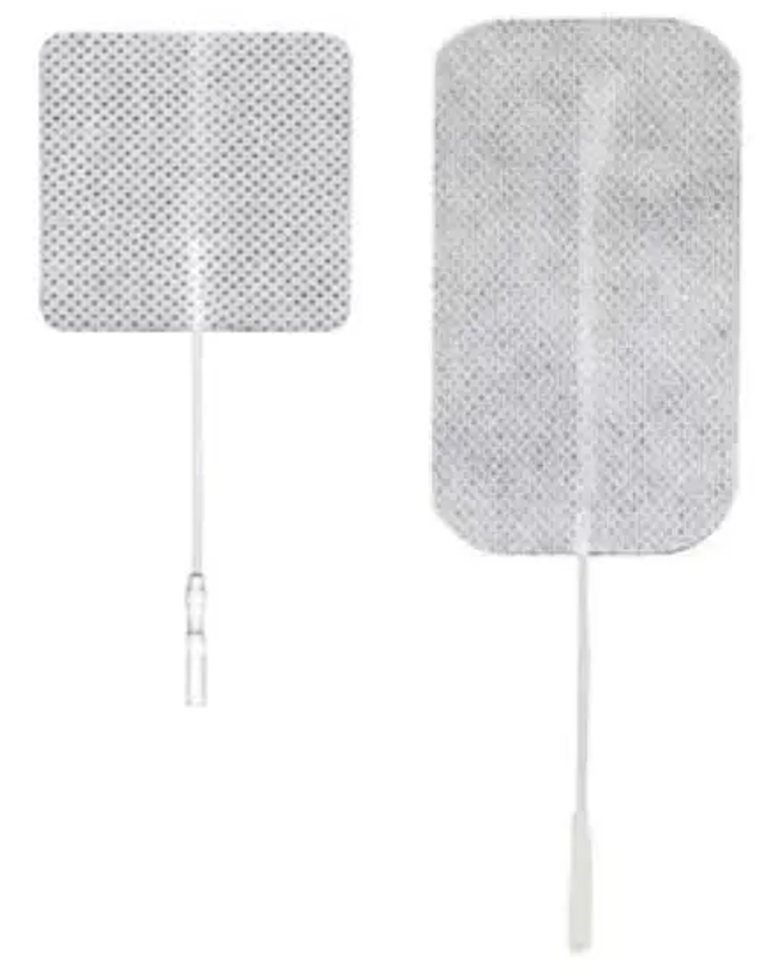
\includegraphics[width=\linewidth]{images/electrodes.png}
    \caption{FES electrodes}
    \label{fig:electrodes}
\end{wrapfigure}

Every stimulated muscle thereby required two electrodes, one active electrode and one reference electrode. Both 5x5cm and 5x9cm electrodes were used for this project (figure \ref{fig:electrodes}), depending on the muscle size. The connection was realized using cables with banana connectors, visible in figure \ref{fig:stimwave}. The chosen electrodes are equiped with adhesive gel creating a relatively stable electrode-tissue interface. 

\subsubsection{Electrode placement}
The placement of electrodes is an critical factor for achieving effective stimulation. It determines the quality of muscle activation the specificity and the comfort for the user. However, the optimal placements for each muscle is highly subject-dependent which makes the process of finding the placements challenging and time consuming.

To establish some form of systematic approach the optimal placements were first found in myself. This involved iteratively adjusting the placement of both the active and reference electrode positions, observing the muscle responses at different amplitudes and the discomfort level until a functional movement was achieved under the pain threshold (maximum tolerable intensity). Physiologically, optimal electrode placement aligns with the motor points of the targeted muscles \todo{source}. Motor points are regions where the motor nerve enters the muscle, resulting in the lowest threshold for activation thus minimizing discomfort and fatigue \todo{source}. To find the optimal placements for each muscle several sources were consulted with the most used source being an atlas of the muscle motor points by A. Botter \cite{botter_atlas_2011}. 

\begin{figure}
    \centering
    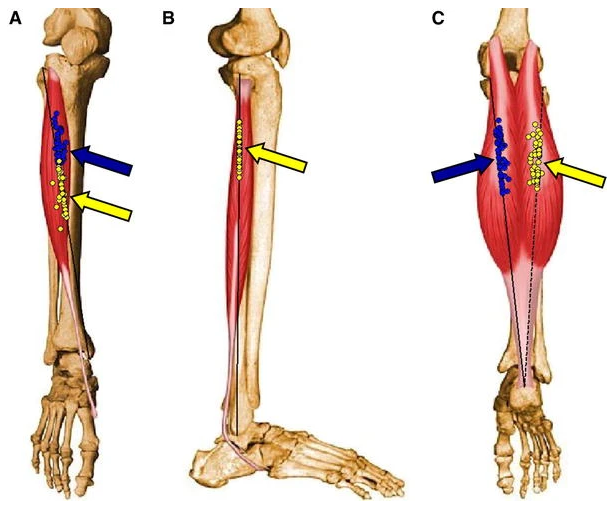
\includegraphics[width=0.6\linewidth]{images/screenshotmotorpoint.png}
    \caption{Example of motor points according to \cite{botter_atlas_2011} for: \textbf{a.} tibialis anterior; \textbf{b.}peroneous longus; \textbf{c.} medial (\textit{blue circles}) and lateral (\textit{yellow circles}) gastrocnemii. }
    \label{fig:motor-points}
\end{figure}

To document the process and provide a reference for future users a series of videos was creates, where each video captures the intended functional movement elicited by optimal stimulation of a muscle. This offers a clear visual benchmark which could then be used when finding the correct placements for new users, thereby maintaining consistency and ensuring that the functional movements are sufficient before moving on to the full gait cycle functional electrical stimulation.

\subsection{Open Loop Stimulation Sequence}
\lhead{Implementation - Open Loop Stimulation Sequence}
The open loop stimulation sequence specifies which muscles should be stimulated, the duration oftheir activation adn the delays between activations. The sequence aims to replicate a single step (gait cycle) for one leg using FES. The final goal is to produce a step that feels and looks natural and is comfortable for the subject while being general enough to work for a variety of subjects.

\subsubsection{Testing the Existing Sequence}
Initially, it was beleived that a working open loop sequence had already been established by a previous student. However upon testing the sequence on two different subject it became clear that the sequence ineffective and did not produce a step. The muscle activation was observed to feel unnatural and uncomfortable and ultimatley failed to pelicate a smooth coordinated movement. It therefore became necessary to dermine whether these issues stemned from errors in the implementation or from issues with the sequence itself.

\todo{figures}

This initial sequence was based on electromyography (EMG) measurements of muscle activation during gait in two healthy subject. Therefore to evalueate the accuracy of the sequence the EMG measurements from the two subjects were compaired against a comprehensice, open-source dataset of EMG activity during gait \cite{camargo_comprehensive_2021}. The discrepancies between the two became immediately apparent. In gait phases where the dataset indicated that certain muscles-such as the vastus medialis, hamstrings,and gluteus maximus-should be largely inactive the EMG measurement from the two subjects showed significant activation. There are several likely causes for these inaccuracies uncluding noise, motion artifacts or the EMG sensors picking up activity from muscles. Since the stimulation sequence was based directly on this flawed data several muscles were being stimulated during periods where they should be entierly inactive. This is what lead to the failure of the sequence in reproducing a natural and functional gait cycle. Having confirmed that the issue lay in the sequence itself, rather than its implementation, the focus was shifted to designing an entirely new stimulation sequence.

\subsubsection{Finding a new sequence}

\textit{Graphical User Interface}

To facilitate the testing and tuning of new stimulation sequences a new graphical user interface (GUI) tab (figure \ref{fig:sequenceGUI})was created. This interface allowed real-time adjustments not only to the durations and delayes but also the sequence of the muscles. This is done by relating each muscle to a specific channel. This significantly accelerated the iterative process of testing and optimizing sequences. 

\begin{figure} [h]
    \centering
    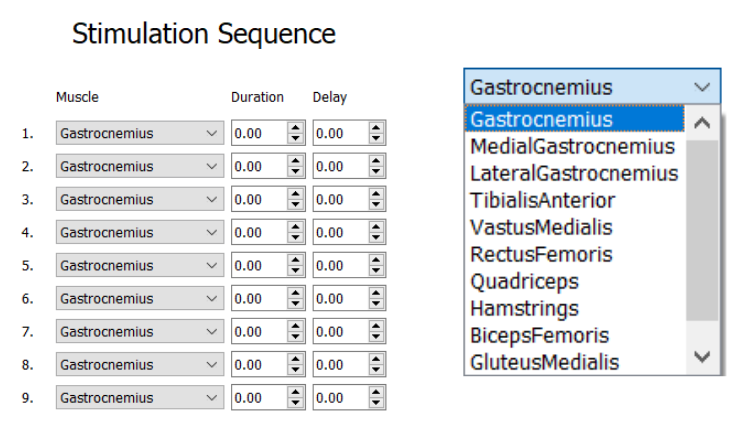
\includegraphics[width=0.8\linewidth]{images/sequenceGUI.png}
    \caption{Graphical user interface for testing new sequences.}
    \label{fig:sequenceGUI}
\end{figure}

\textit{Methodology}

In order to design a new sequence that would be robust literature insights from the literature relating to FES for gait and a seminal text on gait physiology were used. To ensure that the sequence aligned with natural muscle activation patterns, the seminal text \textit{Gait Anlysis: Normal and Pathological function} \cite{perry_gait_2024} was consulted. This book provides comprehensive descriptions of muscle activity throughout the gait cycle with exact start and top percentages of the gait cycle for nearly all lower extremity muscles during gait. However the gait stimulation sequence could not be based only on this. It would be impossible to stimulate every muscle individually as they are activated naturally, there are simply too many muscles and FES does not have the necessary selectivity to accomplish that. Unlike voluntary contractions, which selectively and smoothly activate specific motor units, FES broadly stimulates motor nerves, often activating muscles indiscriminately. Therefore it was necessary to choose only a few muscles to stimulate and to determine this the existing literature relating to FES was examined.

\begin{figure} [h]
    \centering
    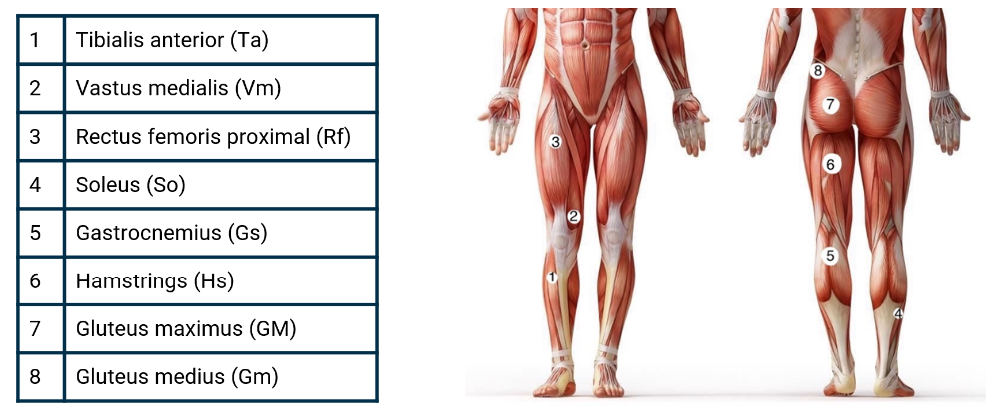
\includegraphics[width=0.85\linewidth]{images/common_muscles.png}
    \caption{Common muscles used for FES driven gait}
    \label{fig:commonMuscles}
\end{figure}

The literature ( \todo{sources}) revealed a large variety in the sequences used in FES gait studies. The timing end exact muscles varied greatly, however, the number of muscles was relatively consistent between four and eight and the tibialis anterior, gastrocnemis and biceps femoris (hamstring) appeared consistently in nearly all implementations. A list and visualization of the most common muscles is shown in figure \ref{fig:commonMuscles}. Several sequences inspired by physiological insights and the literature were tested. 
\newline \newline


\subsubsection{Six muscle Sequence}

First a sequence with six muscles: Tibialis Anterior, Gastrocnemi, Vastus Medialis, Hamstrings, Gastrocnemi and the Gluteus Maximus, was tested. This was the first sequence that produced a step. 

\subsubsection{Five muscle sequence}
The next sequence tested did not include the gluteus maximus, this was done to see whether the gluteus was necessary to stimulate. It had been pointed out by collegues experienced with running FES on patients that patients typically find the stimulation and placement process for the gluteus to be both challenging and uncomfortable. 

The hypothesis was that the gluteus Maximus may not be necessary to stimulate since several studies using FES to produce gait did not include the gluteus muscles ( \cite{aout_effects_2023} \todo{sources}). There are several reasons as to why the gluteus maximus, although important in natural gait, may not be necessary to stimulate. The first is muscle compensation. The gluteus is mostly involved in hip stabilization and hip extension. However the hamstring stimulation provides som hip extension that may be sufficient \todo{source}. The second is that the gluteus is primarily active during activities that require powerful hip extension such as climbing stairs or running \todo{source}. For flat ground however, especially at slower speeds the gluteus may play a smaller role. 

This new sequence also produced a step that did not seem of a lower quality than the sequence that included the gluteus. The stimulation was also noted to be more comfortable without the gluteus, therefore it was decided that the gluteus could be removed from the sequence.



\subsubsection{Four muscle sequence}
Next a sequence without the Rectus Femoris was tested, this was done due to several observations. Firstly, during experiments it was observed that stimulating only the Vastus Medialis led to a full knee extension leading to questions as to why the Rectus Femoris must be stimulated as well. The rectus femoris functions in both hip flexion and knee extension during natural gait, however upon FES stimulation it mostly produces an extension. So a hypothesis was formed that they knee extension needed may be achieved through stimulation of only the Vastus Medialis which focuses solely on knee extension without impacting hip movement. Secondly on experimentation done on myself it proved difficult to find a comfortable electrode placement for rectus femoris, and stimulating the rectus femoris proved to be the most uncomfortable muscle to stimulate. This was also corrobarated as a typical experience among patients by experienced collegues. 
Finally it was observed that there was a large discrepancy between when the Rectus Femoris was being stimulated in the literature compared to when it was active during natural gait according to the physiology. In fact in the literature it was largely being used for knee extension, while physiologically this muscle is mostly active during the initial-swing and mid-swing phases where it provides foot clearance and does not act as an extensor at all. 

When testing a new sequence without the rectus femoris there was no discernible difference between the steps produced when looking at videos of the respective sequences. The sequence also proved to be more comfortable leading to the conclusion that the Rectus Femoris may be removed from the sequence. This sequence ended up being the final sequence chosen, with results on multiple subjects available in the result section on the open loop stimulation sequence.


\subsection{IMU implementation}
\lhead{Implementation - IMU implementation}































%=================================================================
%                           End Document
%=================================================================
\end{document}